\documentclass{famnit-thesis}
% \documentclass[english]{famnit-thesis}       % For english version.
% \documentclass[cover]{famnit-thesis}         % Print the cover page.
% \documentclass[review]{famnit-thesis}        % The review version.
% \documentclass[english,cover]{famnit-thesis} % English version with the cover page.
% etc ...

% The bibliography is generated automatically through BibTex.
% Add the bibliography.bib file with all the bibtex entries.

% Import latex packages.
\usepackage{ccicons} % Include if CC symbols are needed.

% The basic thesis information.
\title
    {Naslov zaključne naloge} % Slovene title.
    {The title of the final project paper} % English title.
    {Naslov v glavi dokumenta.} % Title in the heading (with dot at the end).

\author{Ime}{Priimek}{Priimek I.}
\studyprogram{Računalništvo in informatika}
\mentor{prof. dr. Ime Mentorja}{Ime Mentorja, PhD}
\date{junij}{2023}

% Additional thesis information. Remove if not used.
\comentor{doc. dr. Ime Somentorja}{Ime Somentorja, PhD}
\workingcomentor{dr. Ime Delovnega Somentorja}{Ime Delovnega Somentorja, PhD}

% List of keywords in Slovene and English language.
\keywords
    {beseda 1, beseda 2, beseda 3}
    {keyword 1, keyword2, keyword 3}

% Abstract in Slovene and English language.
\abstract
{
    Izvleček predstavlja kratek, a jedrnat prikaz vsebine
    naloge. V največ 250 besedah študent nakaže problem,
    metode, rezultate, ključne ugotovitve in njihov pomen.
}
{
    The abstract describes the content of the project work in a
    concise way. In no more than 250 words, the student outlines
    the problem, the methods, the results, and the conclusions.
}

% The acknowledgments.
\acknowledgments
{
    Za naslovno stranjo (prva notranja stran), ki je stran s podatki oz. opisom uporabljenih licenc (če je zaključno delo izdano pod licencami), sledi zahvala. V njej se zahvalimo sodelujočim pri zaključni nalogi, osebam ali ustanovam, ki so nam pri delu pomagale ali so delo omogočile. Zahvalimo se lahko tudi mentorju in morebitnemu somentorju.
}

% An optional license page.
\licensepage
{
    ~\vfill\noindent
    To delo je ponujeno pod licenco \emph{Creative Commons Priznanje avtorstva --- Deljenje} pod
    enakimi pogoji 2.5 Slovenija (ali novejšo različico). To pomeni, da se tako besedilo, slike,
    grafi in druge sestavine dela kot tudi rezultati diplomskega dela lahko prosto distribuirajo,
    reproducirajo, uporabljajo, priobčujejo javnosti in predelujejo, pod pogojem, da se jasno
    in vidno navede avtorja in naslov tega dela in da se v primeru spremembe, preoblikovanja
    ali uporabe tega dela v svojem delu, lahko distribuira predelava le pod licenco, ki je enaka
    tej. Podrobnosti licence so dostopne na spletni strani \url{http://creativecommons.si/} ali na
    Inštitutu za intelektualno lastnino, Streliška 1, 1000 Ljubljana.

    \begin{center}
        \Huge\ccbysa
    \end{center}

    \medskip\noindent
    Izvorna koda diplomskega dela, njeni rezultati in v ta namen razvita programska oprema je
    ponujena pod licenco GNU General Public License, različica 3 (alinovejša). To pomeni,
    da se lahko prosto distribuira in/ali predeluje pod njenimi pogoji. Podrobnosti licence so
    dostopne na spletni strani \url{http://www.gnu.org/licenses/}.
} % Slovene version
% \licensepage
{
    ~\vfill\noindent
    This work is offered under the \emph{Creative Commons Attribution-ShareAlike} license version 2.5 Slovenia (or newer). This means that both the text, images, graphics, and other components of the work, as well as the results of the thesis, can be freely distributed, reproduced, used, made available to the public, and modified, provided that the author and title of this work are clearly and visibly attributed. In the case of any changes, transformations, or use of this work in another project, the derivative work can only be distributed under a license that is identical to this one. Detailed information about the license is available on the website \url{http://creativecommons.si/} or at the Institute for Intellectual Property, Streliška 1, 1000 Ljubljana.
    
    \begin{center}
        \Huge\ccbysa
    \end{center}
    
     \medskip\noindent   
    The source code of the thesis, its results, and the software developed for this purpose are offered under the GNU General Public License, version 3 (or newer). This means that they can be freely distributed and/or modified under its terms. Detailed information about the license is available on the website \url{http://www.gnu.org/licenses/}.
} & English version

% The list of abbreviations. Remove if not used.
\abbreviation{SSH}{Secure Shell Protocol}
\abbreviation{SMTP}{Simple Mail Transfer Protocol}

\begin{document}
    % Thesis chapters.
    \chapter{UVOD}

Zaključna naloga je avtorsko delo, s katerim študent dokazuje poglobljeno znanje na širših
strokovnih in znanstvenih področjih, usposobljenost za iskanje novih virov znanja na
določenem strokovnem in znanstvenem področju, za uporabo znanstveno-raziskovalnih
metod v širšem spektru problemov in v novih ali spremenjenih okoliščinah, sposobnost za
prevzemanje odgovornosti za vodenje zahtevnejših delovnih sistemov ter za razvijanje
kritične refleksije.
    \chapter{TEHNIČNI PREDPISI}

Zaključna naloga mora biti napisana v pokončnem formatu A4 (strani bele barve). Po končni potrditvi mentorja, morebitnega somentorja, komisije (če je komisija imenovana, kar je odvisno od določil pravilnika o zaključni nalogi posameznega programa) in potrditve tehnične ustreznosti zaključne naloge, študent odda en izvod v PDF formatu v Referat za
študente. Študent posreduje končni potrjen izvod na e-naslov Referata.

Stran naj bo oblikovana tako, da so robovi široki 2,5 cm, glava besedila pa je 1,5 cm (od vrha strani). Če uporabljena programska oprema, ne omogoča točno takšne nastavitve robov in glave besedila, uporabite najbolj podobno.

Besedilo je praviloma v pisavi Times New Roman, velikosti 12 pt, z obojestransko
poravnavo ter razmikom med vrsticami 1,25. Če uporabljena programska oprema, ne omogoča točno takšne nastavitve pisave, uporabite najbolj podobno.

\emph{Opombe} pod črto (footnotes) se pišejo v velikosti 10 pt.

\section{ŠTEVILČENJE STRANI/LISTOV}

Naslovna stran (Priloga B, Priloga F) ni oštevilčena, čeprav velja kot prva stran. Začetne splošne strani so številčene z rimskimi števili od I dalje – in sicer od naslovne strani do zadnje strani kazal oz. seznama kratic.

Z arabskimi številkami začnemo s poglavjem 1 (npr. Uvod) in končamo s poglavjem Literatura. Številka strani je v desnem zgornjem kotu strani, v tekočem ali sprotnem naslovu.

\emph{Tekoči ali sprotni naslov} (running head ali pagina viva) naj bo velikosti 10 pt in oblikovan po vzorcu te strani.

V kolikor naslov zaključne naloge presega vrstico, slednjega v dogovoru z mentorjem in morebitnim somentorjem primerno okrajšajte z uporabo tropičja. Okrajšani naslov se zapisuje samo v tekočem ali sprotnem naslovu (running head ali pagina viva). Na platnici, naslovni strani in ključni dokumentacijski informaciji zapisujete celoten naslov zaključne
naloge

\section{IZDAJA POD LICENCAMI}

Če študent v soglasju z mentorjem odloči, da zaključno nalogo izda pod licencami, ki ponuja določen del pravic vsem (na primer Creative Commons ali GNU GPL), vključi stran z opisom uporabljenih licenc v uvodnem delu naloge, to je takoj za naslovno stranjo (prva notranja stran).

\section{ZAHVALA}

Za naslovno stranjo (prva notranja stran), ki je stran s podatki oz opisom uporabljenih licenc (če je zaključno delo izdano pod licencami), sledi zahvala. V njej se zahvalimo sodelujočim pri zaključni nalogi, osebam ali ustanovam, ki so nam pri delu pomagale ali so delo omogočile. Zahvalimo se lahko tudi mentorju in morebitnemu somentorju.

\section{KLJUČNA DOKUMENTACIJSKA INFORMACIJA}

Za zahvalo sledi stran s podatki o zaključni nalogi - ključna dokumentacijska informacija (KDI) in key document information — ključna dokumentacijska informacija v angleščini.

\section{KAZALA}

Kazala sledijo ključni dokumentacijski informaciji.
Pripraviti je treba vsa ustrezna kazala v naslednjem vrstnem redu:

\begin{itemize}
\item kazalo vsebine,
\item kazalo preglednic,
\item kazalo slik in grafikonov,
\item kazalo prilog,
\item seznam kratic.
\end{itemize}

\section{ŠTEVILČENJE POGLAVIJ}

Za številčenje poglavij uporabljamo arabska števila in dekadni sistem. Poglavja označujemo s števili od 1 dalje. Za številom ne pišemo pike. Iz velikosti in oblike črk naj bo razvidna hierarhija poglavij.

\medskip\noindent
V nadaljevanju je podan primer številčenja poglavij:

\bigskip\noindent
\begin{tabular}{lll}
poglavja 1, 2, 3 & \large VELIKE ČRKE, KREPKO & (npr. 14 pt) \\
poglavja 1.1, 1.2, 2.1 & \large VELIKE ČRKE & (npr. 14 pt) \\
poglavja 1.1.1, 1.1.2 & Male črke, krepko & (npr. 12 pt) \\
poglavja 1.1.1.1, 1.1.1.2 & Male črke, navadno & (npr. 12 pt)
\end{tabular}

\section{OBLIKOVANJE PREGLEDNIC, SLIK IN GRAFI\-KONOV}

Pri oblikovanju preglednic, slik in grafikonov upoštevajte, da:
\begin{itemize}
\item morajo imeti zaporedno številko in naslov;
\item naslov preglednice;
\item naslov slike ali grafikona.
\end{itemize}

Naslove priporočamo velikosti 10 pt, da se optično ločijo od besedila. Umeščenost naslova preglednice, slike ali grafikona se razlikuje glede na navodila za navajanje virov posameznega študijskega programa.

\section{ZAKLJUČNA NALOGA V ANGLEŠKEM JEZIKU: DALJŠI POVZETEK V SLOVENSKEM JEZIKU}

V kolikor je študentu v skladu s pravili fakultete odobrena priprava zaključne naloge v angleškem jeziku, mora študent pripraviti povzetek naloge v obsegu od 4.000 do 10.000 znakov (s presledki) v slovenskem jeziku. Povzetek naloge v slovenskem jeziku je zadnje poglavje naloge ter je ustrezno oštevilčeno (pred poglavjem Literatura in viri).

\section{LITERATURA IN VIRI}

Vsa literatura in viri uporabljeni v magistrskem delu morajo biti ustrezno citirani. Študenti kršijo postopek priprave zaključnega dela, če prepišejo besedila drugih avtorjev v celoti ali delno in pri tem ne citirajo avtorja (plagiatorstvo) oz. če delo ni rezultat študentovega lastnega dela.

Za sankcioniranje teh kršitev se uporabljajo določila Pravilnika o preverjanju in ocenjevanju znanja na Univerzi na Primorskem in Pravilnika o disciplinski odgovornosti študentov Univerze na Primorskem. Če pravila citiranja in priprave seznama literature niso določena na drugačen način na ravni posameznega študijskega programa (podrobnejša navodila na ravni posameznega oddelka fakultete), se pri citiranju in pripravi seznama literature uporabi spodnja določila.

Reference morajo biti citirane po abecednem redu prvega avtorja in v tekstu zapisane s številko v oglatem oklepaju, npr.: [1], [1, 2], [1, Theorem 1.5], [2, Corollary 9.4].
    \chapter{Metodologija}

\noindent
Graf funkcije (\ref{eqn:saddle}) je prikazan na sliki \ref{fig:plot}.

\begin{equation}
    f(x, y) = x^2 - y^2
    \label{eqn:saddle}
\end{equation}

\begin{figure}[ht]
    \centering
    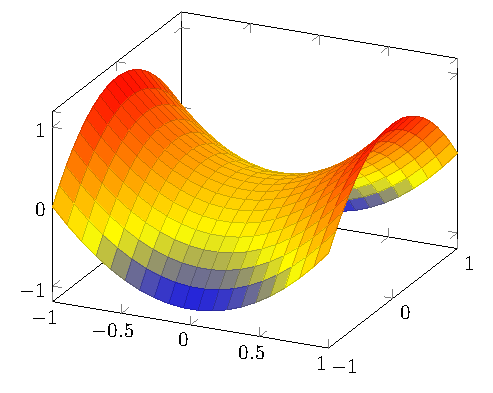
\includegraphics[width=0.6\linewidth]{images/plot.pdf}
    \caption{Graf funkcije $f(x, y) = x^2 - y^2$.}
    \label{fig:plot}
\end{figure}

\begin{table}[ht]
    \centering
    \caption{Nekaj vrednosti funkcije (\ref{eqn:saddle}).}
    \begin{tabular}{|rr|c|}
        \hline
        $x$  & $y$  & $f(x, y)$ \\
        \hline
        $-1$ & $-1$ & $0$ \\
        $-1$ & $0$  & $1$ \\
        $1$ & $0$   & $1$ \\
        \hline
    \end{tabular}
\end{table}

    % English version must also contain an extended Slovene abstract,
    % 4,000 - 10,000 characters including spaces.
    %\input{abstract.tex}

    % Optional appendices. Remove if not used.
    \appendix{A}{Naziv priloge}

Besedilo priloge.

\end{document}
